%----------------------------------------------------------------------------------------
%	PACKAGES AND OTHER DOCUMENT CONFIGURATIONS
%----------------------------------------------------------------------------------------

\documentclass{article}

%%%%%%%%%%%%%%%%%%%%%%%%%%%%%%%%%%%%%%%%%
% Lachaise Assignment
% Structure Specification File
% Version 1.0 (26/6/2018)
%
% This template originates from:
% http://www.LaTeXTemplates.com
%
% Authors:
% Marion Lachaise & François Févotte
% Vel (vel@LaTeXTemplates.com)
%
% License:
% CC BY-NC-SA 3.0 (http://creativecommons.org/licenses/by-nc-sa/3.0/)
% 
%%%%%%%%%%%%%%%%%%%%%%%%%%%%%%%%%%%%%%%%%

%----------------------------------------------------------------------------------------
%	PACKAGES AND OTHER DOCUMENT CONFIGURATIONS
%----------------------------------------------------------------------------------------

\usepackage{amsmath,amsfonts,stmaryrd,amssymb} % Math packages

\usepackage{enumerate} % Custom item numbers for enumerations

\usepackage[ruled]{algorithm2e} % Algorithms

\usepackage[framemethod=tikz]{mdframed} % Allows defining custom boxed/framed environments

\usepackage{float}

\usepackage{listings} % File listings, with syntax highlighting
\lstset{
	basicstyle=\ttfamily, % Typeset listings in monospace font
}

%----------------------------------------------------------------------------------------
%	DOCUMENT MARGINS
%----------------------------------------------------------------------------------------

\usepackage{geometry} % Required for adjusting page dimensions and margins

\geometry{
	paper=a4paper, % Paper size, change to letterpaper for US letter size
	top=2.5cm, % Top margin
	bottom=3cm, % Bottom margin
	left=2.5cm, % Left margin
	right=2.5cm, % Right margin
	headheight=14pt, % Header height
	footskip=1.5cm, % Space from the bottom margin to the baseline of the footer
	headsep=1.2cm, % Space from the top margin to the baseline of the header
	%showframe, % Uncomment to show how the type block is set on the page
}

%----------------------------------------------------------------------------------------
%	FONTS
%----------------------------------------------------------------------------------------

\usepackage[utf8]{inputenc} % Required for inputting international characters
\usepackage[T1]{fontenc} % Output font encoding for international characters

\usepackage{XCharter} % Use the XCharter fonts

%----------------------------------------------------------------------------------------
%	COMMAND LINE ENVIRONMENT
%----------------------------------------------------------------------------------------

% Usage:
% \begin{commandline}
%	\begin{verbatim}
%		$ ls
%		
%		Applications	Desktop	...
%	\end{verbatim}
% \end{commandline}

\mdfdefinestyle{commandline}{
	leftmargin=10pt,
	rightmargin=10pt,
	innerleftmargin=15pt,
	middlelinecolor=black!50!white,
	middlelinewidth=2pt,
	frametitlerule=false,
	backgroundcolor=black!5!white,
	frametitle={Command Line},
	frametitlefont={\normalfont\sffamily\color{white}\hspace{-1em}},
	frametitlebackgroundcolor=black!50!white,
	nobreak,
}

% Define a custom environment for command-line snapshots
\newenvironment{commandline}{
	\medskip
	\begin{mdframed}[style=commandline]
}{
	\end{mdframed}
	\medskip
}

%----------------------------------------------------------------------------------------
%	FILE CONTENTS ENVIRONMENT
%----------------------------------------------------------------------------------------

% Usage:
% \begin{file}[optional filename, defaults to "File"]
%	File contents, for example, with a listings environment
% \end{file}

\mdfdefinestyle{file}{
	innertopmargin=1.6\baselineskip,
	innerbottommargin=0.8\baselineskip,
	topline=false, bottomline=false,
	leftline=false, rightline=false,
	leftmargin=2cm,
	rightmargin=2cm,
	singleextra={%
		\draw[fill=black!10!white](P)++(0,-1.2em)rectangle(P-|O);
		\node[anchor=north west]
		at(P-|O){\ttfamily\mdfilename};
		%
		\def\l{3em}
		\draw(O-|P)++(-\l,0)--++(\l,\l)--(P)--(P-|O)--(O)--cycle;
		\draw(O-|P)++(-\l,0)--++(0,\l)--++(\l,0);
	},
	nobreak,
}

% Define a custom environment for file contents
\newenvironment{file}[1][File]{ % Set the default filename to "File"
	\medskip
	\newcommand{\mdfilename}{#1}
	\begin{mdframed}[style=file]
}{
	\end{mdframed}
	\medskip
}

%----------------------------------------------------------------------------------------
%	NUMBERED QUESTIONS ENVIRONMENT
%----------------------------------------------------------------------------------------

% Usage:
% \begin{question}[optional title]
%	Question contents
% \end{question}

\mdfdefinestyle{question}{
	innertopmargin=1.2\baselineskip,
	innerbottommargin=0.8\baselineskip,
	roundcorner=5pt,
	nobreak,
	singleextra={%
		\draw(P-|O)node[xshift=1em,anchor=west,fill=white,draw,rounded corners=5pt]{%
		Question \theQuestion\questionTitle};
	},
}

\newcounter{Question} % Stores the current question number that gets iterated with each new question

% Define a custom environment for numbered questions
\newenvironment{question}[1][\unskip]{
	\bigskip
	\stepcounter{Question}
	\newcommand{\questionTitle}{~#1}
	\begin{mdframed}[style=question]
}{
	\end{mdframed}
	\medskip
}

%----------------------------------------------------------------------------------------
%	WARNING TEXT ENVIRONMENT
%----------------------------------------------------------------------------------------

% Usage:
% \begin{warn}[optional title, defaults to "Warning:"]
%	Contents
% \end{warn}

\mdfdefinestyle{warning}{
	topline=false, bottomline=false,
	leftline=false, rightline=false,
	nobreak,
	singleextra={%
		\draw(P-|O)++(-0.5em,0)node(tmp1){};
		\draw(P-|O)++(0.5em,0)node(tmp2){};
		\fill[black,rotate around={45:(P-|O)}](tmp1)rectangle(tmp2);
		\node at(P-|O){\color{white}\scriptsize\bf !};
		\draw[very thick](P-|O)++(0,-1em)--(O);%--(O-|P);
	}
}

% Define a custom environment for warning text
\newenvironment{warn}[1][Warning:]{ % Set the default warning to "Warning:"
	\medskip
	\begin{mdframed}[style=warning]
		\noindent{\textbf{#1}}
}{
	\end{mdframed}
}

%----------------------------------------------------------------------------------------
%	INFORMATION ENVIRONMENT
%----------------------------------------------------------------------------------------

% Usage:
% \begin{info}[optional title, defaults to "Info:"]
% 	contents
% 	\end{info}

\mdfdefinestyle{info}{%
	topline=false, bottomline=false,
	leftline=false, rightline=false,
	nobreak,
	singleextra={%
		\fill[black](P-|O)circle[radius=0.4em];
		\node at(P-|O){\color{white}\scriptsize\bf i};
		\draw[very thick](P-|O)++(0,-0.8em)--(O);%--(O-|P);
	}
}

% Define a custom environment for information
\newenvironment{info}[1][Info:]{ % Set the default title to "Info:"
	\medskip
	\begin{mdframed}[style=info]
		\noindent{\textbf{#1}}
}{
	\end{mdframed}
}
 % Include the file specifying the document structure and custom commands

%----------------------------------------------------------------------------------------
%	ASSIGNMENT INFORMATION
%----------------------------------------------------------------------------------------

\title{Homework 1: Lateral Inhibition} % Title of the assignment

\author{Oliver Rutving s164209} % Author name and email address

\date{Introduction to Cognitive Science 02454 --- \today} % University, school and/or department name(s) and a date

%----------------------------------------------------------------------------------------


\begin{document}

\maketitle % Print the title

%----------------------------------------------------------------------------------------
%	PROBLEM 1
%----------------------------------------------------------------------------------------

\section{Exercise 1} % Numbered section
Let $x_1, x_2, x_3$ represent how many deciliters of each product A, B or C should be produced. 
\\
She can sell product A for 60kr per liter, product B for 70kr per liter and product C for 30kr per liter. This gives the objective function $Z=6x_1+7x_2+3x_3$. 
The objective function says that for every dl of product A sold she will profit 6kr. If she sells 2dl of each product, she will earn $Z=6*2+7*2+3*2=32$
\\
Since the DTU student has 7 liters of Ethanol and product A uses 1dl, product B 2dl and product C 1dl, we have the constraint: $x_1+2x_2+x_3\leq 70$
\\
She has 21 liters of apple juice. Product A uses 2dl, product B uses 2dl and product C uses 3dl, which gives the constraint $2x_1+2x_2+3x_3\leq 210$
\\
Lastly, she has 20 liters of Coca-Cola. Product A uses 3dl, product B uses 1dl and product C uses 1dl, which gives the constraint $3x_1+x_2+x3\leq 200$
\\
The constraints and objective function gives the following LP:
\\
\begin{equation*}
    \begin{array}{ll@{}ll}
    \text{Maximize}  & Z=6x_1+7x_2+3x_3\\
                     & \\
    \text{Subject to}& x_1+2x_2+x_3\leq 70\\
                     & 2x_1+2x_2+3x_3\leq 210\\
                     & 3x_1+x_2+x_3\leq 200\\
                     & x_1, x_2, x_3 \geq 0
\end{array}
\end{equation*}
\\
It is informed that for the optimal solution, she only makes product A and product B and that she does not use up all the apple juice.
There are 3 constraints and so there must be 3 basic variables.
Based on this information, it can be concluded that $x_1, x_2$ (product A and B) as well as the slack variable for the second constraint (apple juice) are basic variables. 
This is because $x_1$ and $x_2$ are non-zero in the solution and because the apple juice was not used up (the slack variable is also non-zero)

\vspace{5mm}
Initial system of equations:

\vspace{5mm}
\begin{tabular}{|l|l|l|l l l l l l|l|}
  \hline
  B.V           & Eq. & Z & x1 & x2 & x3 & x4 & x5 & x6 & RHS \\ \hline
  Z             & (0) & 1 & -6 & -7 & -3 & 0  & 0  & 0  & 0   \\ \hline
  $x_4$            & (1) & 0 & 1  & 2  & 1  & 1  & 0  & 0  & 70  \\ \hline
  $x_5$            & (2) & 0 & 2  & 2  & 3  & 0  & 1  & 0  & 210 \\ \hline
  $x_6$            & (3) & 0 & 3  & 1  & 1  & 0  & 0  & 1  & 200 \\ \hline
\end{tabular}
\vspace{5mm}
\\
Using the fundamental insight described above, it is possible to write up the final tabeau. 
The basic variables are $x_1, x_2$ and $x_5$ and so:
\[c_B=[6, 7, 0] \ \ \ \ \ B=
\begin{bmatrix}
  1 & 2 & 0 \\
  2 & 2 & 1 \\
  3 & 1 & 0
\end{bmatrix}
\]

\pagebreak
The values are calculated in Julia like so:

\vspace{5mm}
\begin{file}[Project 1.jl]
	\begin{lstlisting}[language=matlab]
A=[1 2 1; 2 2 3; 3 1 1]
I=[1 0 0; 0 1 0; 0 0 1]
B=[1 2 0; 2 2 1; 3 1 0]
b=[70; 210; 200]
c=transpose([6,7,3])
cB=transpose([6,7,0])
   
cB*inv(B)*A-c
inv(B)*A
cB*inv(B)
inv(B)
cB*inv(B)*b
inv(B)*b    
	\end{lstlisting}
\end{file}


\vspace{5mm}
The optimal tableau becomes:

\vspace{5mm}
\begin{tabular}{|l|l|l|l l l l l l|l|}
  \hline
  B.V           & Eq. & Z & x1 & x2 & x3 & x4 & x5 & x6 & RHS \\ \hline
  Z             & (0) & 1 & 0 & 0 & 1 & 3 & 0 & 1 & 0   \\ \hline
  $x_1$            & (1) & 0 & 1 & 0 & 0.2 & -0.2 & 0 & 0.4 & 66  \\ \hline
  $x_2$            & (2) & 0 & 0 & 1 & 0.4 & 0.6 & 0 & -0.2 & 2 \\ \hline
  $x_5$           & (3) & 0 & 0 & 0 & 1.8 & -0.8 & 1 & -0.4 & 74 \\ \hline
\end{tabular}


\section{Exercise 2} % Numbered section

The third constraint is negative and so: $-x_1+2x_2\geq -2 \Longleftrightarrow x_1-2x_2\leq 2$
The LP is written in augmented form:
\\
\begin{equation*}
    \begin{array}{ll@{}ll}
    \text{Maximize}  & Z=x_1+3x_2&\\
    \text{Subject to}& x1+2x_2+\overline{x}_3 =18\\
                     & -2x_1+x_2+x_4=3\\
                     & x_1-2x_2+x_5=2\\
                     & x_1, x_2, \overline{x_3}, x_4, x_5\geq 0
\end{array}
\end{equation*}
\\
Since there are artificial variables, the two-phase method is used to solve the problem.
The artificial variables are minimized: $min\ Z=\overline{x}_3 \Longleftrightarrow\ max -Z+\overline{x}_3=0$

\vspace{5mm}
\begin{tabular}{|l|l|l|l l l l l|l|}
  \hline
  B.V             & Eq. & Z & $x_1$ & $x_2$ & $\overline{x}_3$ & $x_4$ & $x_5$  & RHS\\ \hline
  Z               & (0) & -1& 0  & 0  & 1  & 0  & 0   & 0  \\ \hline
  $\overline{x}_3$& (1) & 0 & 1  & 2  & 1  & 0  & 0   & 18 \\ \hline
  $x_4$           & (2) & 0 & -2 & 1  & 0  & 1  & 0   & 3  \\ \hline
  $x_5$& (3) & 0 & 1  & -2 & 0  & 0  & 1   & 2 \\ \hline
\end{tabular}

\vspace{5mm}
The tableau is not legal. Row 1 is subtracted from Row 0: 

\vspace{5mm}
\begin{tabular}{|l|l|l|l l l l l|l|l|}
  \hline
  B.V             & Eq. & Z & $x_1$ & $x_2$ & $\overline{x}_3$ & $x_4$ & $x_5$  & RHS & Ratio\\ \hline
  Z               & (0) & -1& -1 & -2 & 0  & 0  & 0   & -18 & \\ \hline
  $\overline{x}_3$& (1) & 0 & 1  & 2  & 1  & 0  & 0   & 18  & 9 \\ \hline
  $x_4$           & (2) & 0 & -2 & 1  & 0  & 1  & 0   & 3   & 3 \\ \hline
  $x_5$           & (3) & 0 & 1  & -2 & 0  & 0  & 1   & 2   & -1\\ \hline
\end{tabular}

\vspace{5mm}
$x_4$ is the leaving variable (because it has the lowest positive ratio) and $x_2$ is the entering variable:

Operations: $R2_{new}=R2/1, R0_{new}=R0+2*R2_{new}, R1_{new}=R1-2*R2_{new}, R3_{new}=R3+2*R2_{new}$

\vspace{5mm}
\begin{tabular}{|l|l|l|l l l l l|l|l|}
  \hline
  B.V             & Eq. & Z & $x_1$ & $x_2$ & $\overline{x}_3$ & $x_4$ & $x_5$  & RHS & Ratio\\ \hline
  Z               & (0) & -1& -5 & 0  & 0  & 2  & 0   & -12 & \\ \hline
  $\overline{x}_3$& (1) & 0 & 5  & 0  & 1  & -2 & 0   & 12  & 12/5\\ \hline
  $x_2$           & (2) & 0 & -2 & 1  & 0  & 1  & 0   & 3   & -3/2\\ \hline
  $x_5$           & (3) & 0 & -3 & 0  & 0  & 2  & 1   & 8   & -8/3\\ \hline
\end{tabular}


\vspace{5mm}
$\overline{x}_3$ is the leaving variable (because it has the lowest positive ratio) and $x_1$ is the entering variable:

Operations: $R1_{new}=R1/5, R0_{new}=R0+5*R1_{new}, R2_{new}=R2+2*R1_{new}, R3_{new}=R3+3*R1_{new}$

\vspace{5mm}
\begin{tabular}{|l|l|l|l l l l l|l|}
  \hline
  B.V             & Eq. & Z & $x_1$ & $x_2$ & $\overline{x}_3$ & $x_4$ & $x_5$  & RHS\\ \hline
  Z               & (0) & -1& 0  & 0  & 1  & 0  & 0   & 0    \\ \hline
  $x_1$           & (1) & 0 & 1  & 0  & 0.2&-0.4& 0   & 2.4  \\ \hline
  $x_2$           & (2) & 0 & 0  & 1  & 0.4& 0.2& 0   & 7.8 \\ \hline
  $x_5$           & (3) & 0 & 0  &  0 & 0.6& 0.8& 1   & 15.2 \\ \hline
\end{tabular}

\vspace{5mm}
There are no negative coefficients in row 0 (the objective row). The variables have been minimized.

The columns of the artificial variables are deleted and the original objective function is inserted:

\vspace{5mm}
\begin{tabular}{|l|l|l|l l l l|l|}
  \hline
  B.V             & Eq. & Z & $x_1$ & $x_2$ & $x_4$ & $x_5$  & RHS\\ \hline
  Z               & (0) & -1& -1 & -3 & 0  & 0   & 0    \\ \hline
  $x_1$           & (1) & 0 & 1  & 0  &-0.4& 0   & 2.4  \\ \hline
  $x_2$           & (2) & 0 & 0  & 1  & 0.2& 0   & 7.8 \\ \hline
  $x_5$           & (3) & 0 & 0  &  0 & 0.8& 1   & 15.2 \\ \hline
\end{tabular}

\vspace{5mm}
The tableau is illegal. Row 1 is added once to row 0 and row 2 is added three times:

\vspace{5mm}
\begin{tabular}{|l|l|l|l l l l|l|}
  \hline
  B.V             & Eq. & Z & $x_1$ & $x_2$ & $x_4$ & $x_5$  & RHS\\ \hline
  Z               & (0) & -1& 0 & 0 & 0.2  & 0   & 25.8    \\ \hline
  $x_1$           & (1) & 0 & 1  & 0  &-0.4& 0   & 2.4  \\ \hline
  $x_2$           & (2) & 0 & 0  & 1  & 0.2& 0   & 7.8 \\ \hline
  $x_5$           & (3) & 0 & 0  &  0 & 0.8& 1   & 15.2 \\ \hline
\end{tabular}

\vspace{5mm}
There are no negative values in the objective row and so the optimal solution is found:

$Z=25.8$ when $(x_2,x_1)=(7.8, 2.4)$

\vspace{10mm}
In figure 1 is the solution space to the problem. 
Neither $x_1$ nor $x_2$ start out as basic variables and so they are both zero: $(x_2,x_1)=(0,0)$.
Notice that $x_1$ is on the second axis and $x_2$ is in the first axis in the graph.
The artificial variable $\overline{x}_3$ needed to be minimized. 
As constraint 1 was the only constraint constaining $\overline{x}_3$, this was the only one that was subtracted from the objective function.
Because $x_2$ had the largest positive coefficient, this was the one chosen as the entering variable.
In figure 1, this is equivalent to traveling along the first axis.
$x_4$ was chosen as the leaving variable as it had the smallest (positive) ratio.
Thus, the first solution to be visited was where the second row (constraint) intersected with the first axis: (3,0)

Next, $\overline{x}_3$ was chosen as the leaving variable and $x_1$ as the entering variable.
The second solution and optimal solution to be visited was where the second row (constraint) intersected with the first row (constraint): (7.8,2.4)

\begin{figure}[H]
  \centering
  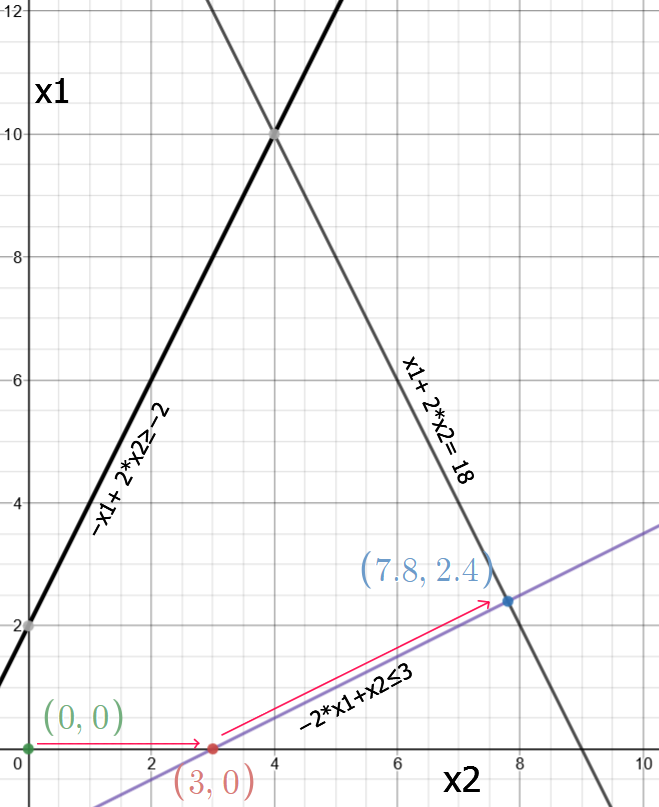
\includegraphics[width=0.6\linewidth]{lpc.PNG}
  \caption{Solution Space}
\end{figure}






\section{Exercise 3} % Numbered section

The problem is written in standard form:
\\
\begin{equation*}
    \begin{array}{ll@{}ll}
    \text{Maximize}  & Z=-2x_1^++2x_1^- -x_2'+2 \\
                     & \\
    \text{Subject to}& -2x_1^++2x_1^- +x_2' \leq 5 \\
                     & x_1^+-x_1^- \leq 5\\
                     & x_1^+-x_1^- +3x_2' \leq 14\\
                     & x^+_1, x^-_1, x_2' \geq 0
\end{array}
\end{equation*}

Initial system of equations:

\vspace{5mm}
\begin{tabular}{|l|l|l|l l l l l l|l|}
  \hline
  B.V           & Eq. & Z & $x_1^+$& $x_1^-$& $x_2'$ & $x_3$ & $x_4$ & $x_5$ & RHS \\ \hline
  Z             & (0) & 1 & 2  & -2 & 1  & 0  & 0  & 0  & 2   \\ \hline
  $x_3$         & (1) & 0 & -2 & 2  & 1  & 1  & 0  & 0  & 5  \\ \hline
  $x_4$         & (2) & 0 & 1  & -1 & 0  & 0  & 1  & 0  & 5 \\ \hline
  $x_5$         & (3) & 0 & 1  & -1 & 3  & 0  & 0  & 1  & 14 \\ \hline
\end{tabular}
\vspace{5mm}
\\

$c, A, B, b$ and $c_B$ are constructed from the initial problem:

$c=[-2, 2, -1]$

$B=[1, 0, 0; 0, 1, 0; 0, 0, 1]$

$b=[5; 5; 14]$

$A=[-2, 2, 1; 1, -1, 0; 1, -1, 3]$

$cB=[0, 0, 0]$

\vspace{5mm}
First is the optimality test:

$cB*inv(B)*A-c=[2, -2, 1]$

-2 is the most negative number, $x_1^-$ is entering the basis

\vspace{5mm}
The minimum ratio test is done to find the leaving variable:

$inv(B)*b=[5, 5, 14]$

$inv(B)*A[:,2]=[2, -1, -1]$

$5/2$ is the only positive ratio and so $x_3$ is chosen as the leaving variable

\vspace{5mm}
$B$ and $c_B$ can now be updated:

$B=[2, 0, 0; -1, 1, 0; -1, 0, 1]$

$cB=[2, 0, 0]$

The optimality test is done again for the second iteration:

$cB*inv(B)*A-c=[0,0,2]$

Since there are no negative values, the optimal solution has been found.

\vspace{5mm}
The optimal tableau:

\vspace{5mm}
\begin{tabular}{|l|l|l|l l l l l l|l|}
  \hline
  B.V           & Eq. & Z & $x_1^+$& $x_1^-$& $x_2'$ & $x_3$ & $x_4$ & $x_5$ & RHS \\ \hline
  Z             & (0) & 1 & 0  & 0  & 2  & 1  & 0  & 0  & 5 \\ \hline
  $x_1^-$       & (1) & 0 & -1 & 1  & 0.5& 0.5& 0  & 0  & 2.5 \\ \hline
  $x_4$         & (2) & 0 & 0  & 0  & 0.5& 0.5& 1  & 0  & 7.5  \\ \hline
  $x_5$         & (3) & 0 & 0  & 0  & 3.5& 0.5& 0  & 1  & 16.5  \\ \hline
\end{tabular}
\vspace{5mm}
\\

The optimal objective value is $Z=c_BB^{-1}b+2=5+2=7$

2 is added as this was the constant in the original objective function.

\vspace{5mm}
The optimal values for $x_1$ and $x_2$ are:
$x_1=-x_1^-=-2.5$ and $x_2=-2*(x_1)-Z=-2*(-2.5)-7=-2$

So the optimal objective value for the original problem is $Z=7$ when $(x_1,x_2)=(-2.5,-2)$




\pagebreak

\section{Exercise 4} % Numbered section

In figure 2 below is the minimum cost flow graph for the problem:

\begin{figure}[H]
  \centering
  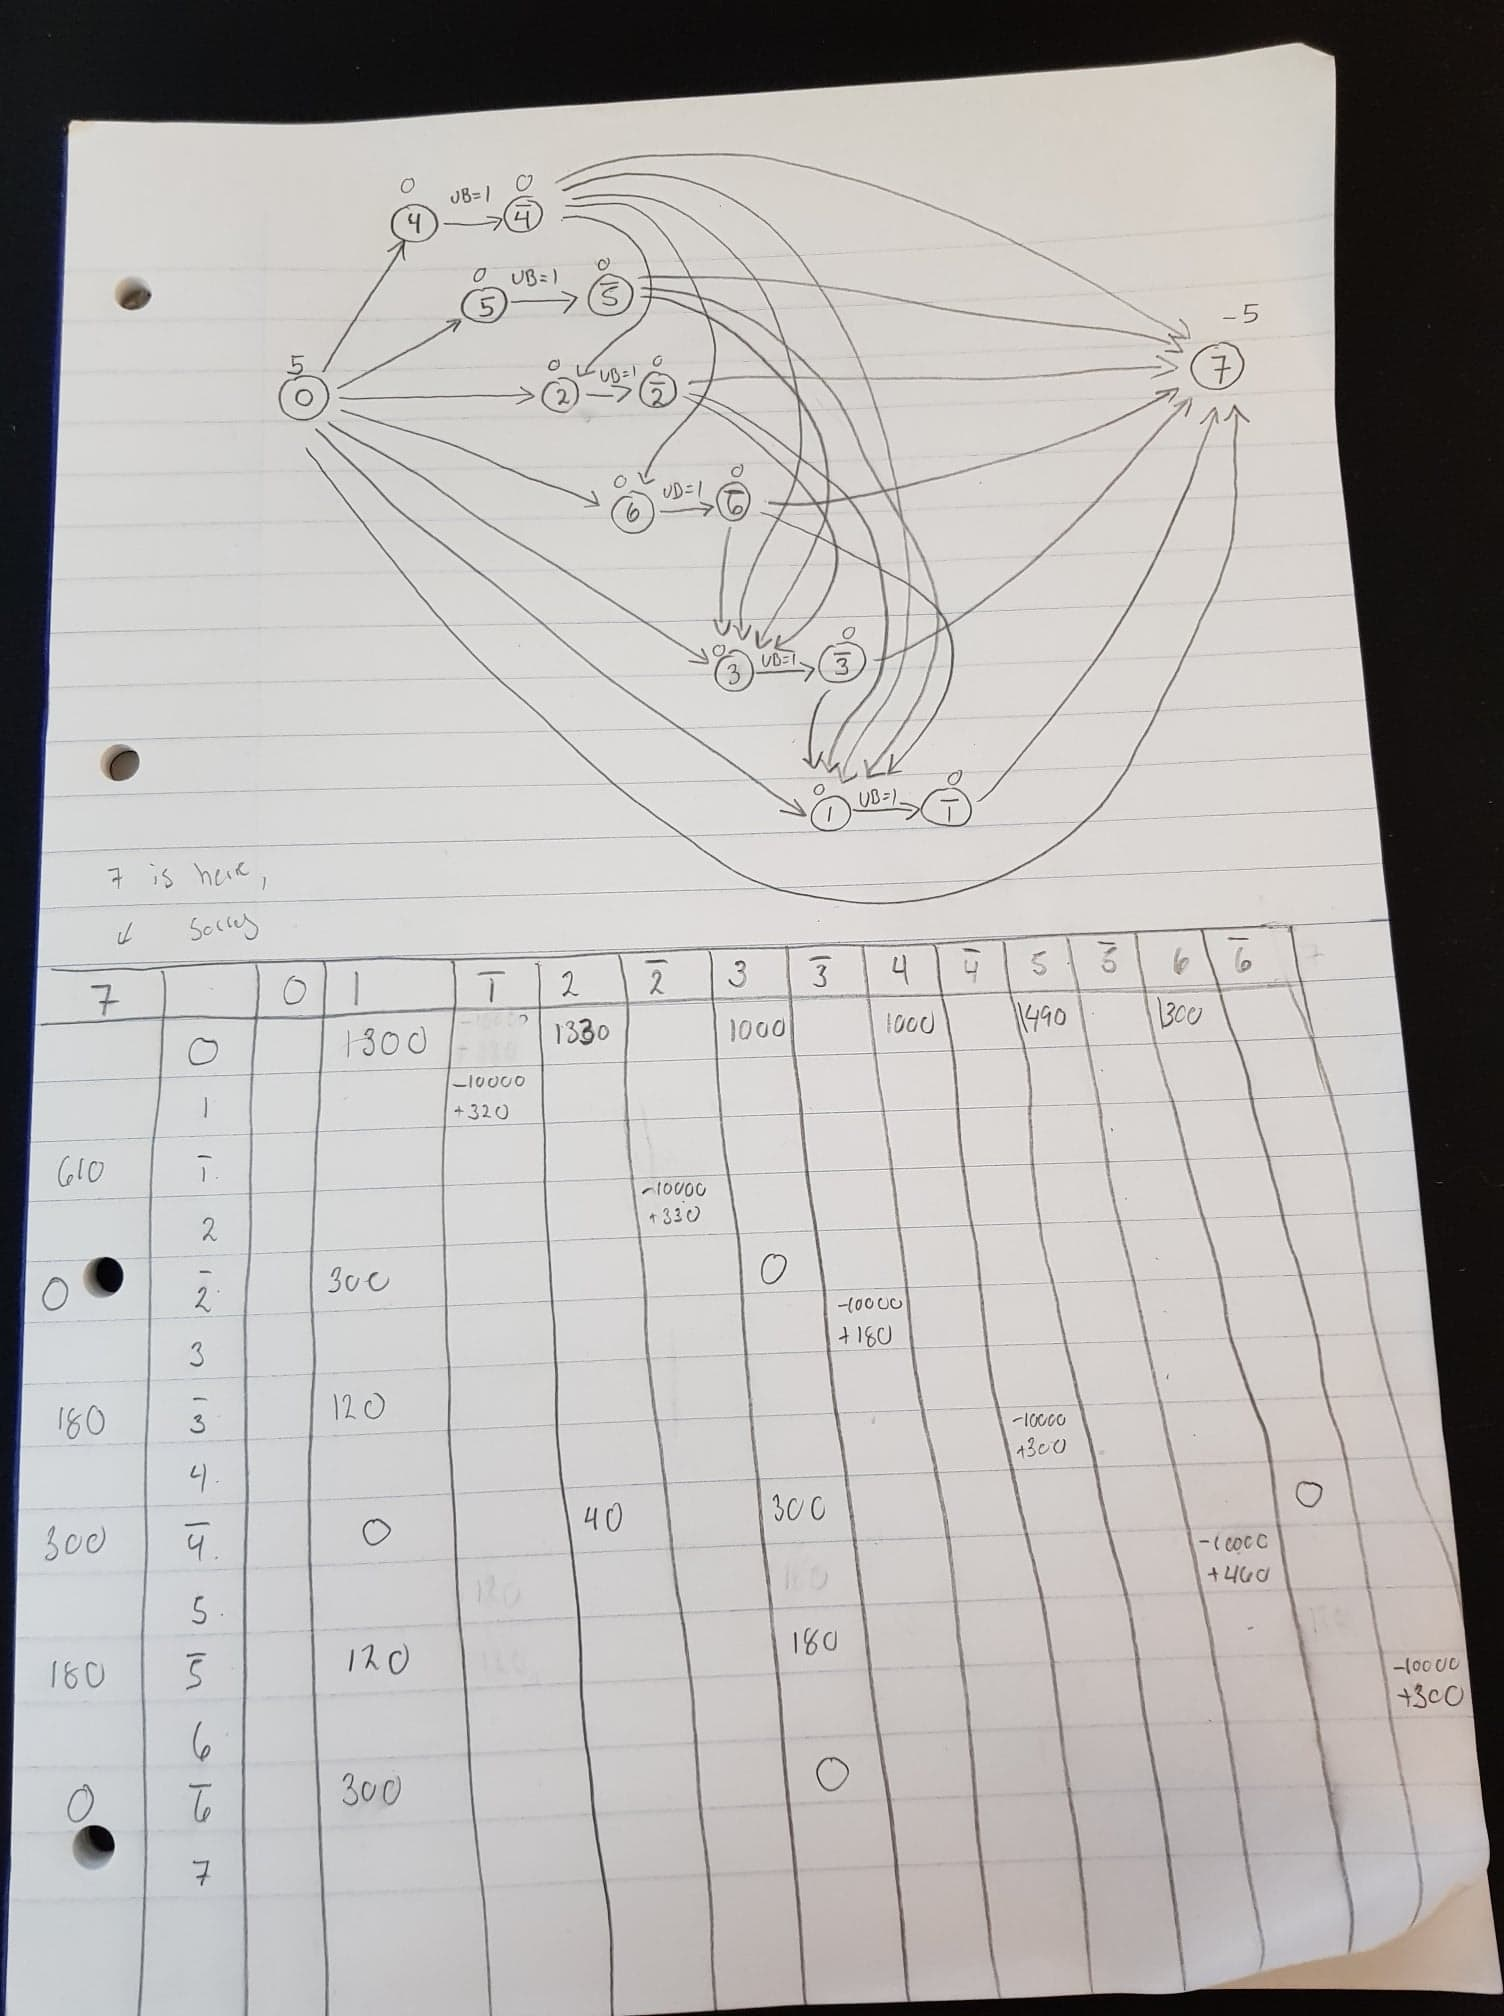
\includegraphics[width=0.9\linewidth]{pic.jpg}
  \caption{Minimum cost flow graph and the cost table}
\end{figure}

Node 0 and 7 represents the bus depot. The node pairs $4\rightarrow\overline{4}$ represents a trip. 
Each trip has an upper bound of 1 since every trip only needs to be done once.
If it is possible for a bus to go from the end location of a trip and to the beginning of another, a line is made from the end node of the first trip to the start node of the other. Below the flow graph is the cost table showing the cost of going from one location to another.

\pagebreak

The problem is setup in julia, refer to $Exercise4.jl$ to see code.

When running the code, the command line shows the following:


% Command-line "screenshot"
\begin{commandline}
	\begin{verbatim}
Flow on arc (1,2) is 1.0
Flow on arc (3,4) is 1.0
Flow on arc (5,6) is 1.0
Flow on arc (7,8) is 1.0
Flow on arc (9,10) is 1.0
Flow on arc (11,12) is 1.0
Flow on arc (13,1) is 0.0
Flow on arc (13,3) is 1.0
Flow on arc (13,5) is 0.0
Flow on arc (13,7) is 1.0
Flow on arc (13,9) is 1.0
Flow on arc (13,11) is 0.0
Flow on arc (13,14) is 2.0
Flow on arc (2,14) is 1.0
Flow on arc (4,5) is 1.0
Flow on arc (4,1) is 0.0
Flow on arc (4,14) is 0.0
Flow on arc (6,1) is 1.0
Flow on arc (6,14) is 0.0
Flow on arc (8,1) is 0.0
Flow on arc (8,3) is 0.0
Flow on arc (8,5) is 0.0
Flow on arc (8,11) is 1.0
Flow on arc (8,14) is 0.0
Flow on arc (10,1) is 0.0
Flow on arc (10,5) is 0.0
Flow on arc (10,14) is 1.0
Flow on arc (12,1) is 0.0
Flow on arc (12,5) is 0.0
Flow on arc (12,14) is 1.0
	\end{verbatim}
\end{commandline}

Interpretation:
3 busses are used. This is seen from the arc (13,14) which is 2 meaning that 2 busses stay at node 0 (location A, the bus depot)

The cost of the solution is -53380. The real cost of the solution is $-53380+60000=6620$ since there are 6 trips and each trip has a bonus of -10000 to make sure all trips are done.

\vspace{5mm}
One bus goes from node 0 to 4 and does trip 4 (since (13,7) and (7,8) is 1). 
It then does trip 6 (since (8,11) and (11, 12) is 1). 
Finally it goes back to the bus depot (since (12, 14) is 1 and 14 represents the end node)
So the first bus goes from location $A\rightarrow E\rightarrow A$ and finishes trip 4 and trip 6.

The price for this trip was $1000+300+300=1600$


\vspace{5mm}
Another bus first does trip 5 and then goes to the bus depot (since (13,9), (9,10), (10,14)=1)
It goes from location $A\rightarrow D\rightarrow B\rightarrow A$ and only finishes trip 5.

The price for this trip was $1000+490+460+180=2130$

\vspace{5mm}
The last bus does trip 2, trip 3 and trip 1. (since (13,3), (3,4), (4,5), (5, 6), (6, 1), (1,2), (2,14) = 1)

It goes from location $A\rightarrow F\rightarrow A\rightarrow B\rightarrow E\rightarrow C\rightarrow A$ and finishes trip 2, 3 and 1.

The price for the trip was $1000+330+330+180+120+320+610=2890$

The price for doing all trips was $1600+2130+2890=6620$ as seen in the objective value.


\vspace{5mm}
\hrulefill 
end of the assignment
\end{document}
